\justifying
\textbf{Цель работы:}
Научиться аппроксимировать функции тригонометрическим многочленом и полиномами Чебышева. Сравнить полученные результаты.

\textbf{Задание:}
Сравнить аппроксимации бесконечно дифференцируемой функции
\begin{equation}\label{task}
    f(x) = A_1 cos(\omega_1 x) + A_2 sin(\omega_2 x) 
\end{equation}
на отрезке $[-1,1]$, полученные с помощью тригонометрического многочлена ряда Фурье
\begin{eqnarray}
    S_N^{(1)}(x) &=& \frac{a_0^{(1)}}{2} + \sum_{n=1}^{N} (a_n^{(1)} cos(\pi n x) + b_n^{(1)} sin(\pi n x), \quad |x| \leq 1, \\
    a_n^{(1)} &=& \int_{-1}^{1} f(x) cos(\pi n x) dx, \quad n = 0,1,...,N, \label{formula1}\\
    b_n^{(1)} &=& \int_{-1}^{1} f(x) sin(\pi n x) dx, \quad n = 0,1,...,N, \label{formula2}
\end{eqnarray}
и аппроксимации Чебышевскими многочленами
\begin{equation}
    S_N^{(2)}(x) = \sum_{n=0}^{N} a_n^{(2)} T_n(x), \quad |x| \leq 1, \quad T_n(x) = cos(n \: arccos \, x).
\end{equation}

\textbf{Ход работы:}

Коэффициенты тригонометрического многочлена ряда Фурье были вычислены по формулам~(\ref{formula1} -- \ref{formula2}). Для вычисления Чебышевских коэффициентов было использовано быстрое дискретное преобразование Фурье по следующим формулам:

\begin{eqnarray}
    a_0^{(2)} &\sim& \frac{1}{N} \sum_{m = 0} ^ {N - 1} f(cos \, t_m) \, dt, \quad t_m = \frac{\pi m}{N}, \\
    a_n^{(2)} &\sim& \frac{2}{N} \sum_{m = 0} ^ {N - 1} f(cos \, t_m) \, cos(n \, t_m), \quad n > 0.
\end{eqnarray}

После реализации программы на Python для функции~(\ref{eq}) получаются следующие графики:
\begin{equation}
    f(x) = cos(x) + 0.3 \cdot sin(4 x) \label{eq}
\end{equation}
\newpage
\begin{figure*}[ht!]
\setlength{\fboxsep}{0pt}%
\setlength{\fboxrule}{0pt}%
\begin{center}
\centering
\begin{minipage}{0.45\textwidth}
\centering
 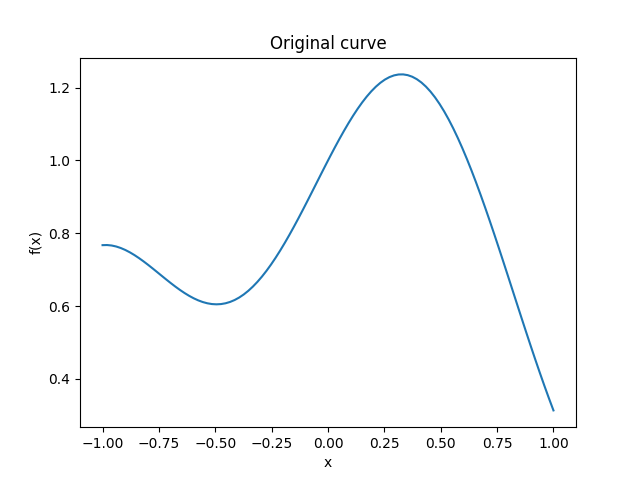
\includegraphics[width=0.95\linewidth]{Figures/Original_curve.png}\\(a)
\end{minipage}
\begin{minipage}{0.45\textwidth}
\centering
 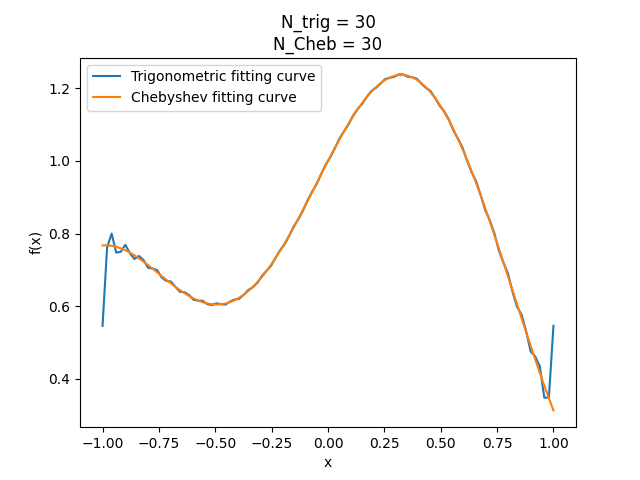
\includegraphics[width=0.95\linewidth]{Figures/Fitting_curves.png}\\(b)
\end{minipage}
\begin{minipage}{0.45\textwidth}
\centering
 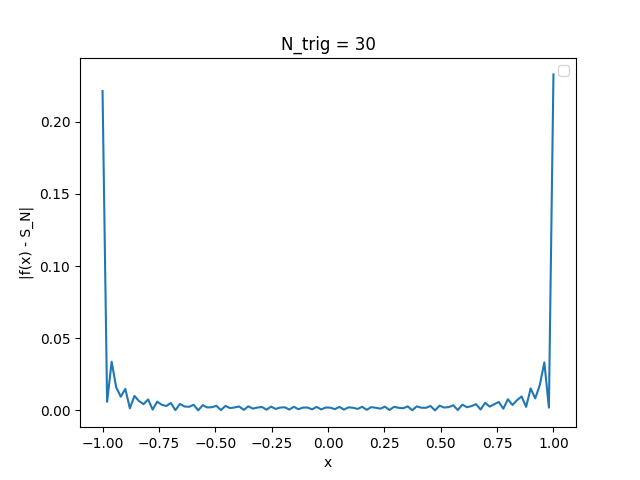
\includegraphics[width=0.95\linewidth]{Figures/Trig_deviation.png}\\(c)
\end{minipage}
\centering
\begin{minipage}{0.45\textwidth}
\centering
 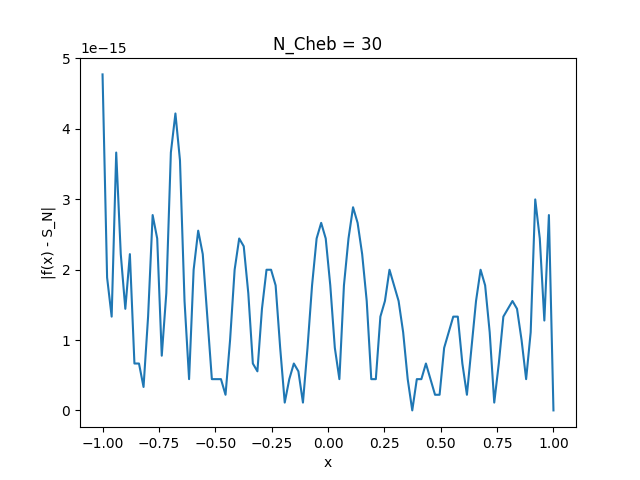
\includegraphics[width=0.95\linewidth]{Figures/Cheb_deviation.png}\\(d)
\end{minipage}
\end{center}
\caption{(a) -- График исходной кривой; (b) -- графики аппроксимирующих кривых; (c) -- график отклонения тригонометрического полинома от исходной функции; (d) -- график отклонения Чебышевского полинома от исходной функции\label{graphs}}
\end{figure*}

Видно, что Чебышевские полиномы намного лучше аппроксимируют исходную функцию, так как относительное отклонение у них порядка $10^{-15}$, в то время как у тригонометрических полиномов отклонение порядка $10^{-1}$.

\textbf{Выводы:}

В настоящей лабораторной работы была произведена аппроксимация бесконечно дифференцируемой функции тригонометрическим многочленом и полиномами Чебышева. После сравнения было выяснено, что полиномы Чебышева аппроксимируют лучше.